 % -*- TeX-engine: xetex; eval: (auto-fill-mode 0); eval: (visual-line-mode 1); -*-
% Compile with XeLaTeX

%%%%%%%%%%%%%%%%%%%%%%%
% To do before class
%%%%%%%%%%%%%%%%%%%%%%%

% Print off Readiness Assessment 1.
% Send email about registering clicker.
% Test run readiness assessment on iClicker.

%%%%%%%%%%%%%%%%%%%%%%%
% Option 1: Slides: (comment for handouts)   %
%%%%%%%%%%%%%%%%%%%%%%%

%\documentclass[slidestop,compress,mathserif,12pt,t,professionalfonts,xcolor=table]{beamer}
%
%% solution stuff
%\newcommand{\solnMult}[1]{
%\only<1>{#1}
%\only<2->{\red{\textbf{#1}}}
%}
%\newcommand{\soln}[1]{\textit{#1}}

%%%%%%%%%%%%%%%%%%%%%%%%%%%%%%%
% Option 2: Handouts, without solutions (post before class)    %
%%%%%%%%%%%%%%%%%%%%%%%%%%%%%%%

 \documentclass[11pt,containsverbatim,handout,xcolor=xelatex,dvipsnames,table]{beamer}

 % handout layout
 \usepackage{pgfpages}
 \pgfpagesuselayout{4 on 1}[letterpaper,landscape,border shrink=5mm]

 % solution stuff
 \newcommand{\solnMult}[1]{#1}
 \newcommand{\soln}[1]{}

%%%%%%%%%%%%%%%%%%%%%%%%%%%%%%%%%%%%
% Option 3: Handouts, with solutions (may post after class if need be)    %
%%%%%%%%%%%%%%%%%%%%%%%%%%%%%%%%%%%%

% \documentclass[11pt,containsverbatim,handout,xcolor=xelatex,dvipsnames,table]{beamer}

% % handout layout
% \usepackage{pgfpages}
% \pgfpagesuselayout{4 on 1}[letterpaper,landscape,border shrink=5mm]

% % solution stuff
% \newcommand{\solnMult}[1]{\red{\textbf{#1}}}
% \newcommand{\soln}[1]{\textit{#1}}

%%%%%%%%%%%%%%%%%%%%%%%%%%%%%%%
% Option 4: Notes Only
%%%%%%%%%%%%%%%%%%%%%%%%%%%%%%%

% % See http://tex.stackexchange.com/questions/114219/add-notes-to-latex-beamer
% \documentclass[10pt,containsverbatim,xcolor=xelatex,dvipsnames,table,notes=only]{beamer}

% % handout layout
% \usepackage{pgfpages}
% \pgfpagesuselayout{2 on 1}[letterpaper, landscape, border shrink=5mm]

% % solution stuff
% \newcommand{\solnMult}[1]{#1}
% \newcommand{\soln}[1]{}

%%%%%%%%%%
% Load style file, defaults  %
%%%%%%%%%%

%%%%%%%%%%%%%%%%
% Themes
%%%%%%%%%%%%%%%%

% See http://deic.uab.es/~iblanes/beamer_gallery/ for mor options

% Style theme
\usetheme{Pittsburgh}

% Color theme
\usecolortheme{seahorse}

% Helvetica Neue Light for most text
\usepackage{fontspec}
\setsansfont{Helvetica Neue Light}

%%%%%%%%%%%%%%%%
% Packages
%%%%%%%%%%%%%%%%

\usepackage{geometry}
\usepackage{graphicx}
\usepackage{amssymb}
\usepackage{epstopdf}
\usepackage{amsmath}  	% this permits text in eqnarray among other benefits
\usepackage{url}		% produces hyperlinks
\usepackage[english]{babel}
\usepackage{colortbl}	% allows for color usage in tables
\usepackage{multirow}	% allows for rows that span multiple rows in tables
\usepackage{color}		% this package has a variety of color options
\usepackage{pgf}
\usepackage{calc}
\usepackage{ulem}
\usepackage{multicol}
\usepackage{textcomp}
\usepackage{listings}
\usepackage{changepage}
\usepackage{tikz}
\usetikzlibrary{trees}		% for probability trees
\usepackage{fancyvrb}	% for colored code chunks
\usepackage{nameref}

%%%%%%%%%%%%%%%%
% Remove navigation symbols
%%%%%%%%%%%%%%%%

\beamertemplatenavigationsymbolsempty
\hypersetup{pdfpagemode=UseNone} % don't show bookmarks on initial view

%%%%%%%%%%%%%%%%
% User defined colors
%%%%%%%%%%%%%%%%

% Pantone 2015 Fall colors
% http://iwork3.us/2015/02/18/pantone-2015-fall-fashion-report/
% update each semester or year

\xdefinecolor{custom_blue}{rgb}{0, 0.32, 0.48} % FROM SPRING 2016 COLOR PREVIEW
\xdefinecolor{custom_darkBlue}{rgb}{0.20, 0.20, 0.39} % Reflecting Pond  
\xdefinecolor{custom_orange}{rgb}{0.96, 0.57, 0.42} % Cadmium Orange
\xdefinecolor{custom_green}{rgb}{0, 0.47, 0.52} % Biscay Bay
\xdefinecolor{custom_red}{rgb}{0.58, 0.32, 0.32} % Marsala

\xdefinecolor{custom_lightGray}{rgb}{0.78, 0.80, 0.80} % Glacier Gray
\xdefinecolor{custom_darkGray}{rgb}{0.35, 0.39, 0.43} % Stormy Weather

%%%%%%%%%%%%%%%%
% Template colors
%%%%%%%%%%%%%%%%

\setbeamercolor*{palette primary}{fg=white,bg= custom_blue}
\setbeamercolor*{palette secondary}{fg=black,bg= custom_blue!80!black}
\setbeamercolor*{palette tertiary}{fg=white,bg= custom_blue!80!black!80}
\setbeamercolor*{palette quaternary}{fg=white,bg= custom_blue}

\setbeamercolor{structure}{fg= custom_blue}
\setbeamercolor{frametitle}{bg= custom_blue!90}
\setbeamertemplate{blocks}[shadow=false]
\setbeamersize{text margin left=2em,text margin right=2em}

%%%%%%%%%%%%%%%%
% Styling fonts, bullets, etc.
%%%%%%%%%%%%%%%%

% title slide
\setbeamerfont{title}{size=\large,series=\bfseries}
\setbeamerfont{subtitle}{size=\large,series=\mdseries}
%\setbeamerfont{institute}{size=\large,series=\mdseries}

% color of alerted text
\setbeamercolor{alerted text}{fg=custom_orange}

% styling of itemize bullets
\setbeamercolor{item}{fg=custom_blue}
\setbeamertemplate{itemize item}{{{\small$\blacktriangleright$}}}
\setbeamercolor{subitem}{fg=custom_blue}
\setbeamertemplate{itemize subitem}{{\textendash}}
\setbeamerfont{itemize/enumerate subbody}{size=\footnotesize}
\setbeamerfont{itemize/enumerate subitem}{size=\footnotesize}

% styling of enumerate bullets
\setbeamertemplate{enumerate item}{\insertenumlabel.}
\setbeamerfont{enumerate item}{family={\fontspec{Helvetica Neue}}}
\setbeamerfont{enumerate subitem}{family={\fontspec{Helvetica Neue}}}
\setbeamerfont{enumerate subsubitem}{family={\fontspec{Helvetica Neue}}}

% make frame titles small to make room in the slide
\setbeamerfont{frametitle}{size=\small} 

% set Helvetica Neue font for frame and section titles
\setbeamerfont{frametitle}{family={\fontspec{Helvetica Neue}}}
\setbeamerfont{sectiontitle}{family={\fontspec{Helvetica Neue}}}
\setbeamerfont{section in toc}{family={\fontspec{Helvetica Neue}}}
\setbeamerfont{subsection in toc}{family={\fontspec{Helvetica Neue}}, size=\small}
\setbeamerfont{footline}{family={\fontspec{Helvetica Neue}}}
\setbeamerfont{subsection in toc}{family={\fontspec{Helvetica Neue}}}
\setbeamerfont{block title}{family={\fontspec{Helvetica Neue}}}

%%%%%%%%%%%%%%%%
% New fonts accessed by fontspec package
%%%%%%%%%%%%%%%%

% Monaco font for code
\newfontfamily{\monaco}{Monaco}

%%%%%%%%%%%%%%%%
% Color text commands
%%%%%%%%%%%%%%%%

%orange
\newcommand{\orange}[1]{\textit{\textcolor{custom_orange}{#1}}}

% yellow
\newcommand{\yellow}[1]{\textit{\textcolor{yellow}{#1}}}

% blue
\newcommand{\blue}[1]{\textit{\textcolor{blue}{#1}}}

% green
\newcommand{\green}[1]{\textit{\textcolor{custom_green}{#1}}}

% red
\newcommand{\red}[1]{\textit{\textcolor{custom_red}{#1}}}

% dark gray
\newcommand{\darkgray}[1]{\textit{\textcolor{custom_darkGray}{#1}}}

% light gray
\newcommand{\lightgray}[1]{\textit{\textcolor{custom_lightGray}{#1}}}

% pink
\newcommand{\pink}[1]{\textit{\textcolor{pink}{#1}}}


%%%%%%%%%%%%%%%%
% Custom commands
%%%%%%%%%%%%%%%%

% empty box for probability tree frame
\newcommand{\emptybox}[2]{
	\fbox{ \begin{minipage}{#1} \hfill\vspace{#2} \end{minipage} }
}

% cancel
\newcommand{\cancel}[1]{%
    \tikz[baseline=(tocancel.base)]{
        \node[inner sep=0pt,outer sep=0pt] (tocancel) {#1};
        \draw[red, line width=0.5mm] (tocancel.south west) -- (tocancel.north east);
    }%
}

% degree
\newcommand{\degree}{\ensuremath{^\circ}}

% cite
\newcommand{\ct}[1]{
\vfill
{\tiny #1}}

% Note
\newcommand{\Note}[1]{
\rule{2.5cm}{0.25pt} \\ \textit{\footnotesize{\textcolor{custom_red}{Note:} \textcolor{custom_darkGray}{#1}}}}

% Remember
\newcommand{\Remember}[1]{\textit{\scriptsize{\textcolor{custom_red}{Remember:} #1}}}

% links: webURL, webLink
\newcommand{\webURL}[1]{\urlstyle{same}{\textit{\textcolor{custom_blue}{\url{#1}}}}}
\newcommand{\webLink}[2]{\href{#1}{\textcolor{custom_blue}{{#2}}}}

% mail
\newcommand{\mail}[1]{\href{mailto:#1}{\textit{\textcolor{custom_blue}{#1}}}}

% highlighting: hl, hlGr, mathhl
\newcommand{\hl}[1]{\textit{\textcolor{custom_blue}{#1}}}
\newcommand{\hlGr}[1]{\textit{\textcolor{custom_green}{#1}}}
\newcommand{\mathhl}[1]{\textcolor{custom_blue}{\ensuremath{#1}}}

% example
\newcommand{\ex}[1]{\textcolor{blue}{{{\small (#1)}}}}

% two col: two columns
\newenvironment{twocol}[4]{
\begin{columns}[c]
\column{#1\textwidth}
#3
\column{#2\textwidth}
#4
\end{columns}
}

% slot (for probability calculations)
\newenvironment{slot}[2]{
\begin{array}{c} 
\underline{#1} \\ 
#2
\end{array}
}

% pr: left and right parentheses
\newcommand{\pr}[1]{
\left( #1 \right)
}

%%%%%%%%%%%%%%%%
% Custom blocks
%%%%%%%%%%%%%%%%

% activity: less commonly used
\newcommand{\activity}[2]{
\setbeamertemplate{itemize item}{{{\small\textcolor{custom_orange}{$\blacktriangleright$}}}}
\setbeamercolor{block title}{fg=white, bg=custom_orange}
\setbeamerfont{block title}{size=\small}
\setbeamercolor{block body}{fg=black, bg=custom_orange!20!white!80}
\setbeamerfont{block body}{size=\small}
\begin{block}{Activity: #1}
\setlength\abovedisplayskip{0pt}
#2
\end{block}
}

% app: application exercise
\newcommand{\app}[2]{
\setbeamercolor{block title}{fg=white,bg=custom_green}
\setbeamercolor{block body}{fg=black,bg=custom_green!20!white!80}
\begin{block}{{\small Application exercise: #1}}
#2
\end{block}
}

% disc: discussion question
\newcommand{\disc}[1]{
\vspace*{-2ex}
\setbeamercolor{block body}{bg=custom_blue!25!white!80, fg=custom_blue!55!black!95}
\begin{block}{\vspace*{-3ex}}
#1
\end{block}
\vspace*{-1ex}
}

% clicker: clicker question
\newcommand{\clicker}[1]{
\setbeamercolor{block title}{bg=custom_blue!80!white!50,fg=custom_blue!30!black!90}
\setbeamercolor{block body}{bg=custom_blue!20!white!80,fg=custom_blue!30!black!90}
\begin{block}{\vspace*{-0.2ex}{\footnotesize Clicker question}\vspace*{-0.2ex}}
#1
\end{block}
}

% formula
\newcommand{\formula}[2]{
\setbeamercolor{block title}{bg=custom_blue!40!white!60,fg=custom_blue!55!black!95}
\begin{block}{{\small#1}}
#2
\end{block}
}

% code
\newcommand{\Rcode}[1]{
{\monaco {\footnotesize \textcolor{custom_darkBlue}{#1}}}
}

% output
\newcommand{\Rout}[1]{
{\monaco {\footnotesize \textcolor{custom_darkGray}{#1}}}
}

%%%%%%%%%%%%%%%%
% Change margin
%%%%%%%%%%%%%%%%

\newenvironment{changemargin}[2]{%
\begin{list}{}{%
\setlength{\topsep}{0pt}%
\setlength{\leftmargin}{#1}%
\setlength{\rightmargin}{#2}%
\setlength{\listparindent}{\parindent}%
\setlength{\itemindent}{\parindent}%
\setlength{\parsep}{\parskip}%
}%
\item}{\end{list}}

%%%%%%%%%%%%%%%%
% Footnote
%%%%%%%%%%%%%%%%

\long\def\symbolfootnote[#1]#2{\begingroup%
\def\thefootnote{\fnsymbol{footnote}}\footnote[#1]{#2}\endgroup}

%%%%%%%%%%%%%%%%
% Graphics
%%%%%%%%%%%%%%%%

\DeclareGraphicsRule{.tif}{png}{.png}{`convert #1 `dirname #1`/`basename #1 .tif`.png}

%%%%%%%%%%%%%%%%
% Slide number
%%%%%%%%%%%%%%%%

\setbeamertemplate{footline}{%
    \raisebox{5pt}{\makebox[\paperwidth]{\hfill\makebox[20pt]{\color{gray}
          \scriptsize\insertframenumber}}}\hspace*{5pt}}

          
%%%%%%%%%%%%%%%%
% Remove page numbers
%%%%%%%%%%%%%%%%

\newcommand{\removepagenumbers}{% 
  \setbeamertemplate{footline}{}
}

%%%%%%%%%%%%%%%%
% TOC slides
%%%%%%%%%%%%%%%%

\setbeamertemplate{section in toc}{\inserttocsectionnumber.~\inserttocsection}
\setbeamertemplate{subsection in toc}{$\qquad$\inserttocsubsectionnumber.~\inserttocsubsection \\}

\AtBeginSection[] 
{ 
  \addtocounter{framenumber}{-1} 
  % 
  {\removepagenumbers 
  {\small
    \begin{frame}<beamer> 
    \frametitle{Outline} 
    \tableofcontents[currentsection] 
  \end{frame} 
  } 
  }
} 

\AtBeginSubsection[] 
{ 
  \addtocounter{framenumber}{-1} 
  % 
  {\removepagenumbers 
  {\small
    \begin{frame}<beamer> 
    \frametitle{Outline} 
    \tableofcontents[currentsection,currentsubsection] 
  \end{frame} 
  } 
  }
}
% You cannot use numbers when defining variables.  
% Hence the use of letters, A, B, C, etc.

% Course Name
\newcommand{\CourseName}{Sta 101 - Fall 2015}
\newcommand{\InstituteName}{Duke University, Department of Statistical Science}

% Personal Info
\newcommand{\FirstName}{Mine}
\newcommand{\LastName}{\c{C}etinkaya-Rundel}
\newcommand{\OfficeHours}{Tue + Thur 4:30-6pm}
\newcommand{\OfficeHoursLocation}{Old Chem 213}

% Electronic Info
\newcommand{\PersonalSite}{http://stat.duke.edu/~mc301}
\newcommand{\CourseSite}{http://bit.ly/sta101_f15}
\newcommand{\Email}{mine@stat.duke.edu}

% TAs
\newcommand{\TAA}{Erika Ball}
\newcommand{\TAB}{David Clancy}
\newcommand{\TAC}{Reuben McCreanor}
\newcommand{\TAD}{Anne Driscoll}
\newcommand{\TAE}{Megan Robertson}

% Exam Dates
\newcommand{\ExamADate}{Mon, Oct 5}
\newcommand{\ExamBDate}{Mon, Nov 9}
\newcommand{\FinalDate}{Thur, Dec 10 (2-5pm)}


% ALT ALT
% % You cannot use numbers when defining variables.  
% Hence the use of letters, A, B, C, etc.

% Personal Info
\newcommand{\FirstName}{Anthea}
\newcommand{\LastName}{Monod}
\newcommand{\OfficeHours}{TBA}
\newcommand{\OfficeHoursLocation}{TBA}

% Electronic Info
\newcommand{\PersonalSite}{TBA}
\newcommand{\CourseSite}{TBA}
\newcommand{\Email}{TBA}

% TAs
\newcommand{\TAA}{TBA}
\newcommand{\TAB}{TBA}
\newcommand{\TAC}{TBA}
\newcommand{\TAD}{TBA}
\newcommand{\TAE}{TBA}

% Exam Dates
\newcommand{\ExamADate}{TBA}
\newcommand{\ExamBDate}{TBA}
\newcommand{\FinalDate}{TBA}



%%%%%%%%%%%
% Cover slide info    %
%%%%%%%%%%%

\title{Unit 2: Probability and distributions}
\subtitle{4. Binomial distribution}
\author{\CourseName}
\date{}
\institute{\InstituteName}


%%%%%%%%%%%%%%%%%%%%%%%%%
% Begin document and set Helvetica Neue font   %
%%%%%%%%%%%%%%%%%%%%%%%%%

\begin{document}
\fontspec[Ligatures=TeX]{Helvetica Neue Light}

%%%%%%%%%%%%%%%%%%%%%%%%%%%%%%%%%%%

% Title Page

\begin{frame}[plain]

\titlepage

\vfill

{\scriptsize \webLink{\PersonalSite}{Dr. \LastName{}} \hfill Slides posted at  \webURL{\CourseSite}}

\addtocounter{framenumber}{-1} 

\end{frame}

%%%%%%%%%%%%%%%%%%%%%%%%%%%%%%%%%%%%

\section{Housekeeping}

%%%%%%%%%%%%%%%%%%%%%%%%%%%%%%%%%%%%

\begin{frame}
\frametitle{Announcements}

\begin{itemize}

\item Project 1 questions?

\item PS2 due Friday night, PA2 due Sunday night

\item RA3 on Monday

\end{itemize}

\end{frame}

%%%%%%%%%%%%%%%%%%%%%%%%%%%%%%%%%%%%

\section{Main ideas}

%%%%%%%%%%%%%%%%%%%%%%%%%%%%%%%%%%%%

\subsection{Binomial distribution is used for calculating the probability of exact number of successes for a given number of trials}
\label{mi1}

%%%%%%%%%%%%%%%%%%%%%%%%%%%%%%%%%%%%

\begin{frame}
\frametitle{High-speed broadband connection at home in the US}

\begin{center}
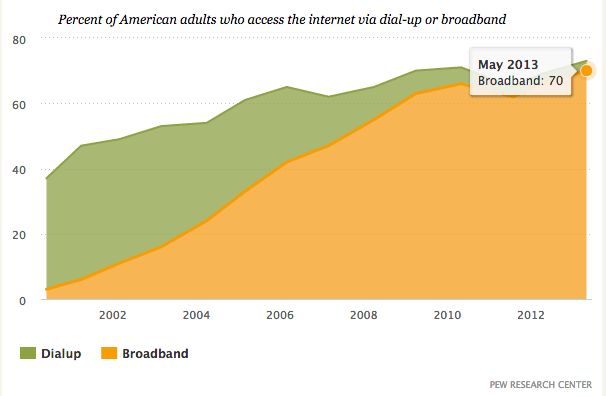
\includegraphics[width=0.6\textwidth]{figures/pew_internet_access}
\end{center}

\pause

\begin{itemize}
\item Each person in the poll be thought of as a \hl{trial}
\pause
\item A person is labeled a \hl{success} if s/he has high-speed broadband connection at home, \hl{failure} if not
\pause
\item Since 70\% have high-speed broadband connection at home, \hl{probability of success} is \hl{p = 0.70}
\end{itemize}

\end{frame}

% %%%%%%%%%%%%%%%%%%%%%%%%%%%%%%%%%%%

\begin{frame}
\frametitle{Considering many scenarios}

\disc{Suppose we randomly select three individuals from the US, what is the probability that exactly 1 has high-speed broadband connection at home?}

Let's call these people Anthony (A), Barry (B), Cam (C). Each one of the three
scenarios below will satisfy the condition of ``exactly 1 of them says Yes'': \\
\vspace{0.25cm}
\pause
\begin{changemargin}{+1.5cm}{+0cm}
{\footnotesize
\begin{enumerate}
\item[Scenario 1:] $\slot{0.70}{\text{(A) \red{yes}}} \times \slot{0.30}{\text{(B) no}} \times \slot{0.30}{\text{(C) no}} \approx 0.063$
\pause
\item[Scenario 2:]  $\slot{0.30}{\text{(A) no}} \times \slot{0.70}{\text{(B) \red{yes}}} \times \slot{0.30}{\text{(C) no}} \approx 0.063$
\pause
\item[Scenario 3:]  $\slot{0.30}{\text{(A) no}} \times \slot{0.30}{\text{(B) no}} \times \slot{0.70}{\text{(C) \red{yes}}} \approx 0.063$
\end{enumerate}
}
\end{changemargin}
\pause
The probability of exactly one 1 of 3 people saying Yes is the sum of all of these probabilities.
\[ 0.063 + 0.063 + 0.063 = 3 \times 0.063 = 0.189 \]

\end{frame}

%%%%%%%%%%%%%%%%%%%%%%%%%%%%%%%%%%%

\begin{frame}
\frametitle{Binomial distribution}

The question from the prior slide asked for the probability of given number of successes, \mathhl{k}, in a given number of trials, \mathhl{n}, ($k = 1$ success in $n = 3$ trials), and we calculated this probability as
\[ \#~of~scenarios \times P(single~scenario) \]

\pause

\begin{itemize}

\item $P(single~scenario) = p^k~(1-p)^{(n-k)}$ \\
{\tiny probability of success to the power of number of successes, probability of failure to the power of number of failures}

\pause

\item number of scenarios: ${n \choose k} = \frac{n!}{k! (n - k)!}$

\end{itemize}

\pause
$\:$ \\

The \hl{Binomial distribution} describes the probability of having exactly $k$
successes in $n$ independent trials with probability of success $p$.

\end{frame}

%%%%%%%%%%%%%%%%%%%%%%%%%%%%%%%%%%%

\begin{frame}[fragile]
\frametitle{Binomial distribution (cont.)}

\[P(k~successes~in~n~trials) = {n \choose k}~p^k~(1-p)^{(n-k)} \] 

\pause

\Note{You can also use R for the calculation of number of scenarios:}
{\footnotesize
\begin{Verbatim}[frame=single, formatcom=\color{blue}]
> choose(5,3)
\end{Verbatim}
}
{\footnotesize
\begin{Verbatim}[frame=single, formatcom=\color{gray}]
[1] 10
\end{Verbatim}
}
\pause
\Note{And to compute probabilities}
{\footnotesize
\begin{Verbatim}[frame=single, formatcom=\color{blue}]
> dbinom(1, size = 3, prob = 0.7)
\end{Verbatim}
}
{\footnotesize
\begin{Verbatim}[frame=single, formatcom=\color{gray}]
[1] 0.189
\end{Verbatim}
}

\end{frame}

%%%%%%%%%%%%%%%%%%%%%%%%%%%%%%%%%%%

\begin{frame}
\frametitle{Properties of the choose function}

\clicker{Which of the following is false?}

\begin{enumerate}[(a)]
\item There are $n$ ways of getting 1 success in $n$ trials, ${n \choose 1} = n$.
\item There is only 1 way of getting $n$ successes in $n$ trials, ${n \choose n} = 1$.
\item There is only 1 way of getting $n$ failures in $n$ trials, ${n \choose 0} = 1$.
\item \solnMult{There are $n-1$ ways of getting $n-1$ successes in $n$ trials, ${n \choose n-1} = n-1$.}
\end{enumerate}

\end{frame}

%%%%%%%%%%%%%%%%%%%%%%%%%%%%%%%%%%%

\begin{frame}

\clicker{Which of the following is not a condition that needs to be met for the binomial distribution to be applicable?}

\begin{enumerate}[(a)]
\item the trials must be independent
\item the number of trials, $n$, must be fixed
\item each trial outcome must be classified as a \textit{success} or a \textit{failure}
\item \solnMult{the number of desired successes, $k$, must be greater than the number of trials}
\item the probability of success, $p$, must be the same for each trial
\end{enumerate}

\end{frame}

%%%%%%%%%%%%%%%%%%%%%%%%%%%%%%%%%%%

\begin{frame}
\frametitle{}

\clicker{According to the results of the Pew poll suggesting that 70\% of Americans have high-speed broadband connection at home, is the probability of exactly 2 out of 15 randomly sampled Americans having such connection at home pretty high or pretty low?}

\begin{enumerate}[(a)]
\item pretty high
\item \solnMult{pretty low}
\end{enumerate}

\end{frame}

%%%%%%%%%%%%%%%%%%%%%%%%%%%%%%%%%%%%

\begin{frame}

\clicker{According to the results of the Pew poll 70\% of Americans have high-speed broadband connection at home, what is the probability that exactly 2 out of 15 randomly sampled Americans have such connection at home?}

\begin{enumerate}[(a)]
\item $0.70^{2} \times 0.30^{13}$

\item ${2 \choose 15} \times 0.70^{2} \times 0.30^{13}$

\item \solnMult{${15 \choose 2} \times 0.70^{2} \times 0.30^{13}$} \soln{\red{\only<2>{$ = \frac{15!}{13! \times 2!} \times  0.70^{2} \times 0.30^{13} = 105 \times  0.70^{2} \times 0.30^{13} = 8.2e-06$}}}

\item ${15 \choose 2} \times 0.70^{13} \times 0.30^2$

\end{enumerate}

\end{frame}

%%%%%%%%%%%%%%%%%%%%%%%%%%%%%%%%%%%

\subsection{Expected value and standard deviation of the binomial can be calculated using its parameters n and p}
\label{mi2}

%%%%%%%%%%%%%%%%%%%%%%%%%%%%%%%%%%%%

\begin{frame}
\frametitle{Expected value and standard deviation of binomial}

\disc{According to the results of the Pew poll suggestion that 70\% of Americans have high-speed broadband connection at home, among a random sample of 100 Americans, how many would you expect to have such connection at home?}

\pause

\begin{itemize}

\item $100 \times 0.70 = 70$
\pause
\begin{itemize}
\item Or more formally, $\mu = np = 100 \times 0.7 = 7$
\end{itemize}

\pause

\item But this doesn't mean in every random sample of 100 Americans exactly 70 will have high-speed broadband connection at home. In some samples there will be fewer of those, and in others more. How much would we expect this value to vary?
\pause
\begin{itemize}
\item $\sigma = \sqrt{np(1-p)} = \sqrt{100 \times 0.70 \times 0.30} \approx  4.58$
\end{itemize}

\end{itemize}

\Note{Mean and standard deviation of a binomial might not always be whole numbers, and that is alright, these values represent what we would expect to see on average.}

\end{frame}


%%%%%%%%%%%%%%%%%%%%%%%%%%%%%%%%%%%

\subsection{Shape of the binomial distribution approaches normal when the S-F rule is met}
\label{mi3}

%%%%%%%%%%%%%%%%%%%%%%%%%%%%%%%%%%%%

\begin{frame}
\frametitle{Shape of the binomial distribution}

\vfill

\begin{center}
\webURL{https://gallery.shinyapps.io/dist_calc/}
\end{center}
\vfill

\pause

You can use the normal distribution to approximate binomial probabilities when
the sample size is large enough.

\hfill \\

\pause

\hl{S-F rule:} 
The sample size is considered large enough if the expected number of successes and failures are both at least 10
\[ np \ge 10 \qquad \text{ and } \qquad n(1-p) \ge 10 \]

\end{frame}

%%%%%%%%%%%%%%%%%%%%%%%%%%%%%%%%%%%

\begin{frame}
\frametitle{}

\clicker{Below are four pairs of Binomial distribution parameters. Which distribution's shape can be approximated by the normal distribution?}

\begin{enumerate}[(a)]
\item \solnMult{$n = 25, p = 0.45$}
\item $n = 100, p = 0.95$
\item $n = 150, p = 0.05$
\item $n = 500, p = 0.015$
\end{enumerate}

\end{frame}


%%%%%%%%%%%%%%%%%%%%%%%%%%%%%%%%%%%%

\begin{frame}[fragile]
\frametitle{}

\disc{What is the probability that among a random sample of 1,000 Americans at
least three-fourths have high-speed broadband connection at home?}

\vspace{-0.5cm}
\pause

\[ Binom(n = 1000, p = 0.7) \]
\vspace{-1cm}

\pause

{\small \[ P(K \ge 750) = P(K = 750) + P(K = 751) + P(K = 752) + \cdots + P(K = 1000) \]}

\pause

\begin{enumerate}

\item Using R:
{\footnotesize
\begin{Verbatim}[frame=single, formatcom=\color{blue}]
> sum(dbinom(750:1000, size = 1000, prob = 0.7))
\end{Verbatim}
}
{\footnotesize
\begin{Verbatim}[frame=single, formatcom=\color{gray}]
[1] 0.00026
\end{Verbatim}
}

\pause

\item Using the normal approximation to the binomial: Since we have at least expected successes
$(1000 \times 0.7 = 700)$ and 10 expected failures $(1000 \times 0.3 = 300)$,

\begin{align*}
Binom&(n = 1000, p = 0.7) \sim \\
&N(\mu = 1000 \times 0.7, \sigma = \sqrt{1000 \times 0.7 \times 0.3}) 
\end{align*}

\end{enumerate}

\end{frame}

%%%%%%%%%%%%%%%%%%%%%%%%%%%%%%%%%%%%

\begin{frame}

\vfill

\app{2.4 Binomial distribution}{See course website for details.}

\vfill

\end{frame}

%%%%%%%%%%%%%%%%%%%%%%%%%%%%%%%%%%%%

% \begin{frame}
% \frametitle{Binomial $\rightarrow$ normal}

% \vfill

% \disc{Why do we care?}

% \vfill

% \end{frame}

%%%%%%%%%%%%%%%%%%%%%%%%%%%%%%%%%%%%

\section{Summary}

%%%%%%%%%%%%%%%%%%%%%%%%%%%%%%%%%%%%

\begin{frame}
\frametitle{Summary of main ideas}

\vfill

\begin{enumerate}

\item \nameref{mi1}

\item \nameref{mi2}

\item \nameref{mi3}

\end{enumerate}

\vfill

\end{frame}

%%%%%%%%%%%%%%%%%%%%%%%%%%%%%%%%%%%

\end{document}